% This file was created by tikzplotlib v0.8.1.
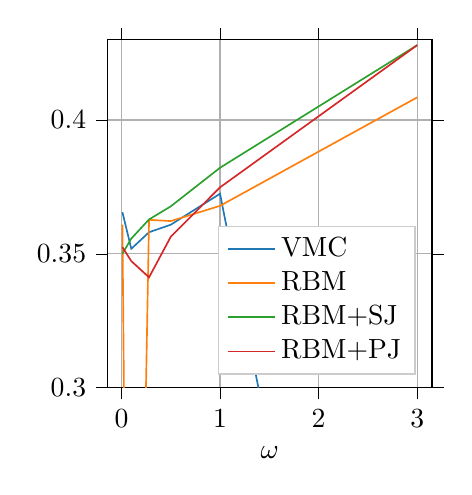
\begin{tikzpicture}

\definecolor{color0}{rgb}{0.12156862745098,0.466666666666667,0.705882352941177}
\definecolor{color1}{rgb}{1,0.498039215686275,0.0549019607843137}
\definecolor{color2}{rgb}{0.172549019607843,0.627450980392157,0.172549019607843}
\definecolor{color3}{rgb}{0.83921568627451,0.152941176470588,0.156862745098039}

\begin{axis}[
legend cell align={left},
legend style={at={(0.34,0.465)}, anchor=north west, draw=white!80.0!black},
tick align=outside,
tick pos=both,
x grid style={white!69.01960784313725!black},
xlabel={\(\displaystyle \omega\)},
xmajorgrids,
xmin=-0.1395, 
xmax=3.1495,
width=5.7cm,
height=6cm,
xtick style={color=black},
y grid style={white!69.01960784313725!black},
%ylabel={\(\displaystyle \langle\mathcal{V}_{ext}\rangle/\langle\mathcal{H}\rangle\)},
ymajorgrids,
ymin=0.30, ymax=0.43,
ytick style={color=black}
]
\addplot [semithick, color0]
table {%
0.01 0.3655571123
0.1 0.351891245
0.28 0.35808008
0.5 0.36087632
1 0.372448783
3 0
};
\addlegendentry{VMC}
\addplot [semithick, color1]
table {%
0.01 0.360945794
0.1 0
0.28 0.3627089294
0.5 0.362241038
1 0.36794137
3 0.408474015
};
\addlegendentry{RBM}
\addplot [semithick, color2]
table {%
0.01 0.350056099
0.1 0.355701411
0.28 0.362851591
0.5 0.36773785
1 0.382174013
3 0.427978032
};
\addlegendentry{RBM+SJ}
\addplot [semithick, color3]
table {%
0.01 0.352495974
0.1 0.347294071
0.28 0.341215239
0.5 0.356358962
1 0.374845451
3 0.4279780324
};
\addlegendentry{RBM+PJ}
\end{axis}

\end{tikzpicture}